\documentclass[10pt]{article}
\usepackage{graphicx}
\usepackage{xeCJK}
\usepackage{placeins}
\usepackage{float}
\usepackage{amsmath}
\setCJKmainfont{MS Mincho} % for \rmfamily
\setCJKsansfont{MS Gothic} % for \sffamily
\graphicspath{ {../image/} }
\renewcommand{\figurename}{図}
\renewcommand{\tablename}{表}

\title{Assignment 2}

\author{Phusaeng Natthaphat (04B23054)}
\date{2026年4月28日}


\begin{document}

\maketitle


\section{課題}
\subsection{Setup}
　次の微分方程式を数値的に解きたい。
\begin{equation}
    \begin{split}
        m\dfrac{dv(t)}{dt}&=-\zeta v(t)\\
        v(0)&=10a\zeta/m
    \end{split}
\end{equation}
まずは解析的に解きましょう。1階の微分方程式なので、導出までもなく、解が直ちに
\begin{equation}
    v(t)=\dfrac{10a\zeta}{m}\exp(-\frac{\zeta}{m}t)
\end{equation}
だと分かる。次のように無次元化する。
\begin{equation}
    \begin{split}
        t&=t_0\tilde{t}\\
        v&=\frac{a}{t_0}\tilde{v}\\
        t_0&=\frac{m}{\zeta}
    \end{split}
\end{equation}
$\sim$がついている量は無次元である。無次元化された解析解は
\begin{equation}
    \tilde{v}(\tilde{t})=10\exp(-\tilde{t})
\end{equation}
となる。\\
　いろいろな時間ステップ$\Delta \tilde{t}(=\Delta t/t_0)$を選び、Euler法を用いて$t\in[0,10^4t_0]$の範囲で計算してみる。

\subsection{結果}
\begin{figure}[p]
    \centering
    \makebox[\textwidth][c]{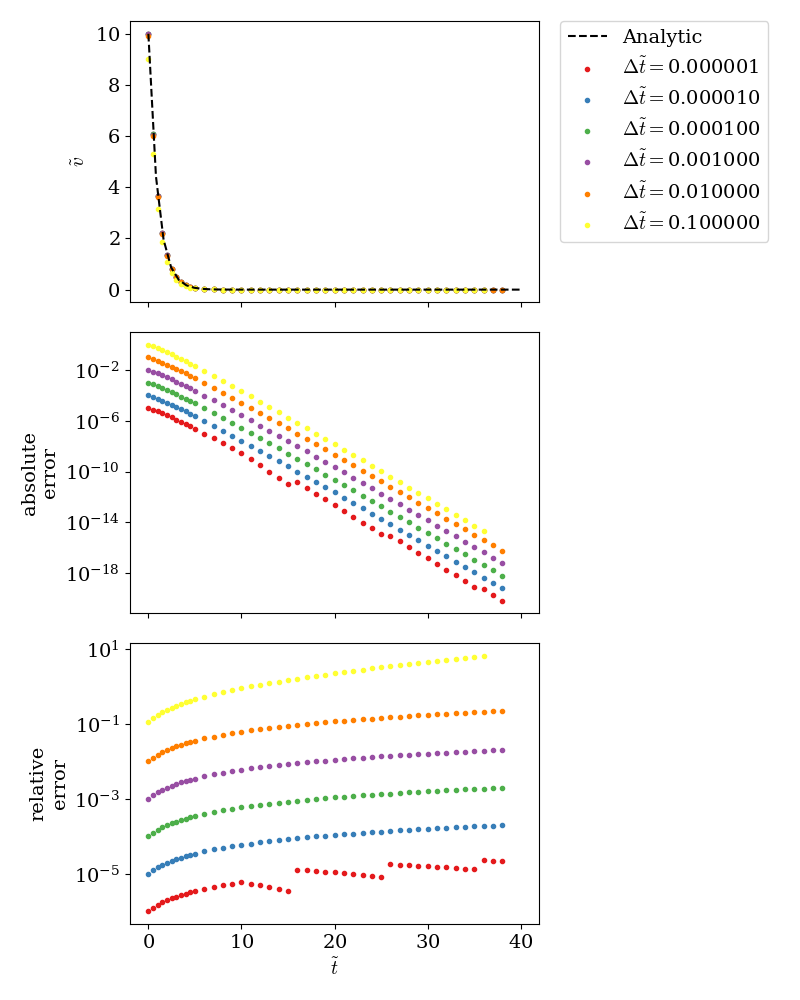
\includegraphics[height=\textheight]{v.png}}
    \caption{$\tilde{v}$ from calculation}
    \label{fig:v}
\end{figure}
　数値計算解と解析解を比較して、absolute errorとrelative errorをプロットする。$\Delta \tilde{t}$を
小さくすれば相対誤差を抑えることができ、一方、$\Delta \tilde{t}$を大きくすぎると誤差が大きくなる。図\ref{fig:v}を見ると、
$\Delta \tilde{t}=0.1$にすると、最終的の誤差が$10\%$もする。

\newpage
\subsection{考察}
　$0<\tilde{t}<10^4$の範囲で計算することは最初の目的でしたが、実際には$\tilde{t}\sim40$しかたどり着かない。
なぜならば、得られた $\tilde{v}$の値が \texttt{double} の最小単位 \texttt{DBL\_EPSILON} $(=2^{-52}\sim2.2\times10^{-16})$より小さいので、
それ以上の精度は記述できないという制限があるから。\\
　続いて、誤差と時間ステップの関係を調べてみよう。得られた数値計算からデータを適当にとり、その値の誤差を計算し、
グラフにしてみる。ただし、横軸は時間ステップ$\Delta \tilde{t}$とする。
\begin{figure}[H]
    \centering
    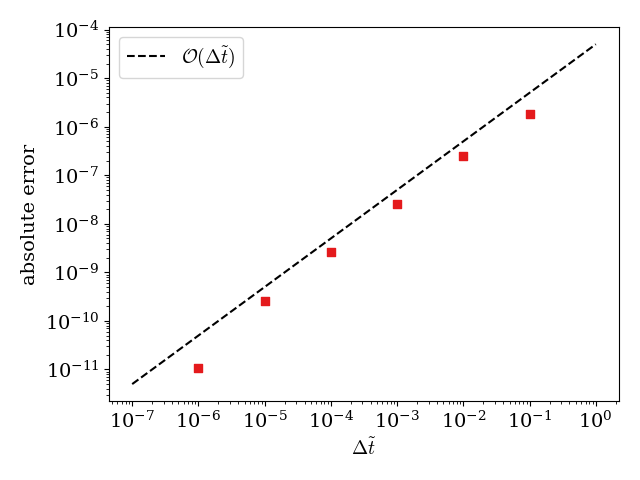
\includegraphics[width=\textwidth]{dt.png}
    \caption{誤差と時間ステップの関係}
    \label{fig:dt}
\end{figure}
　図\ref{fig:dt}から分かるように、誤差は確かに$\mathcal{O}(\Delta \tilde{t})$のオーダーである。
\end{document}